\chapter{Discussion}

The EWC paper is currently one of the most known approaches for overcoming catastrophic forgetting.
Their paper shows that it performs good on a permuted MNIST dataset with three sequential learning tasks.
\newline
Sadly the paper just delivers main facts and ideas behind the EWC solution.
It leaves some important facts for understading their approaches and test benchmarks.
They do show the main idea, formula and advanatges by using them.
But they do not explain why they are using the FIM, in fact just the diagonal of the FIM.
Moreover, they leave out helpful formulas.
Their FIM is not documented and they leave out deeper calculation insights for their idea.
Even an code base is not available.
In the appendix are some parameters of their benchmarks documented.
But their benachmarks for superviseed learning (Figure \ref{fig:ewc_permuted_example}) on the mnist dataset are not reproducible.
They do not present a solution for a reasonable lambda value, learning rate or iterations for the second task.
Therefore, this article had to come up with its own benachmarks.
The benchmarks refer to the report \cite{cf_application_oriented_study} which include an application-oriented study on the EWC algorithm.
The network was given three hidden layers with 800 neurons.
This feature base is a proven structure for the mnist problem.
The iterations and batch sizes are chosen from the study \cite{cf_application_oriented_study}.
This article increased the iterations for the permuted benchmark to analyze the surpassing of the $T_2$ accuracy to the complete dataset.
lambda was default set to $\lambda = \frac{1}{learning \: rate \: T_2}$.

Currently there are multiple implementations of EWC available.
Most of them are created with PyTorch, a similar open-source machine learning library to Tensorflow.
But there are two solutions implemented in Tensorflow and available on Github
\footnote[1]{\url{https://github.com/ariseff/overcoming-catastrophic}}
\footnote[2]{\url{https://github.com/stokesj/EWC}}.
Both show a solution for an permuted mnist on supervised learning but not a disjoint mnist.
The more popular implementation\footnotemark[1] modifies the original algorithm.
For the FIM calulation it does not use the given labels from the dataset.
It generates new labels based on a randomization of the softmax probabilities.
% Moreover, the CrossEntropy loss funtion is not properly used for calculating the gradients.
% They avoid to negate the log from CE
The second implementation \footnotemark[2] is used in the report \cite{cf_application_oriented_study}.
As discovered in Section \ref{project_review_improvements} it built a workaround to be able to perform per-gradient calculations in Tensorflow.
This code base was the inspiration for the default lambda value.
\newline
The reimplementation of EWC in Python and Tensorflow for this article omits these drawbacks and enables the algorithm for the modification \ref{project_review_improvements}.

The baseline showed that the EWC algorithm works with the three benchmarks.
This EWC algorithm (Figures \ref{fig:ewc_d9-1}, \ref{fig:ewc_d5-5}, \ref{fig:ewc_p10-10}) shows that it reduces catastrophic forgetting (Figure \ref{fig:catastrophic_forgetting_example}).
But it does not solve catastrophic forgetting for these benachmarks on the MNIST dataset.
\newline
The application-oriented study \cite{cf_application_oriented_study} discovered that EWC is in some way effective against CF for simple SLTs (D9-1 benchmark), but ineffective against CF for more complex problems (D5-5 benchmark) \cite{cf_application_oriented_study}.
The complete dataset of their simple case (D9-1) has an accuracy after the second task of 71\% and a peak of 99\% \cite{cf_application_oriented_study}.
The results of this article (Figure \ref{fig:ewc_d9-1}) are with 85\% at the end and a peak of 93\% on the complete dataset similar to the paper.
The case of D5-5 they can not register any sign of learning.
The second task has a end result of 31\% with a peak of 50\% \cite{cf_application_oriented_study}.
In comparison to these results, the benchmarks in this article (Figure \ref{fig:ewc_d5-5}) show that there is a learning happending.
This benchmark substantiates an end result of 79\% with an peak of 82\%.
The thrid permuted benchmark in the reference paper \cite{cf_application_oriented_study} shows a peak of 100\% and an end result of 98\% at the second task training.
The result of this article is slightly lower with 95\%.
\newline
It is interesting, that the benchmark types D9-1 and D5-5 with the implementation of this article just work with a lot lower learning rate of 0.00001 for $T_2$.
The learning rate of $T_1$ however is constantly 0.001.
\newline
The comparison of $T_2$ in Figure \ref{fig:ewc_d5-5} and $T_1$ in Figure \ref{fig:ewc_p10-10} shows that in the D5-5 benchmark it would be much easier to just train a new model with the complete mnist dataset.
Because of the same iterations, batch size and a smaller learning rate of $T_1$ (in Figure \ref{fig:ewc_p10-10}) the perfromance of training the complete dataset instead of retraining with the EWC algorithm would increase the accuracy by 15.37\%.
But these benchmarks are just a small representation of the problems in a largely scaled environment for models and datasets.
In this case mnist just provides a simplification of the problem to be able to test an algorithm.
And it gives the ability to test several different parameters in a short amount of time and computation power.
So these benchmarks help to get a better understanding of the algorithm.
If the EWC would be used in real-worls scenarios, it would be used in cases, where the multitask learning (Figure \ref{fig:intro_motivation_multitask_learning_paradigm}) is not an option.

For the implementation of the EWC algorithm with Python and Tensorflow exist multiple ways.
The attached codebase \footnote{\url{https://github.com/florianwiech/incremental-machine-learning}} tried multiple implementations.
First implementations dealt with own coded dataset, iterator and network classes.
The advantage is that the developer has full control over the complete code.
A big disadvantage is though, that other developers need a lot of effort to understand the code.
This is why a developers should stick to given helper classes of the included frameworks.
Most of the time they present a good documentation and other developers who know the framework are able to understand the code quiet quickly.
Because of that reason the code was converted to built-in Tensorflow classes like the Dataset, Iterator and autoloading of the MNIST dataset.
This code sticks as close as possible to the Tensorflow provided classes and Low-Level API.
But along the way of converting the code to the Tensorflow classes, the developer of the code just lost a lot of control and the ability to see what exactly being calculated by just looking at the code.
This is a huge disadvantage with the built-in classes of Tensorflow.
\newline
Through the own implementation, the option between a FIM calculation and the modification is straightforward by adjusting the "batch\_fisher" variable.
Since both computations with a batch size of 1 are the same, the modification is applied when the fisher batch size is higher than one.

The modification of the FIM was tested in the experiments.
The comparison between the baseline benchmarks and experiments with the modification look encouraging.
\newline
The \textbf{benchmark type D9-1} in the experiment Figure \ref{fig:exp_d9-1_bs1k} compared to the baseline Figure \ref{fig:ewc_d9-1} show that the algorithm does work with this modification.
This modification did not compute per-gradient, but rather averaged gradients over 1,000 samples.
The complete dataset has in Figure \ref{fig:ewc_d9-1} a peak of 93.43\% and an end accuracy of 85.81\% compared to Figure \ref{fig:exp_d9-1_bs1k} with a peak of 93.26\% and at the end 85.01\%.
\newline
To get deeper insights, Figure \ref{fig:dis_d91} shows the maximum calculated gradients of each layer in the matrices after the $T_1$ training.
The Parameters represent the set of weights and biases of theta for each layer.
It shows only the maximum values, because the minimum values are all approximatively zero and not  meaningful.
It is interesting that in this case the maximum gradients of the modification are often nearly 200\% the size of the FIM gradients.
But the learning of $T_2$ is in both cases similar.

\begin{figure}[H]
    \centering
    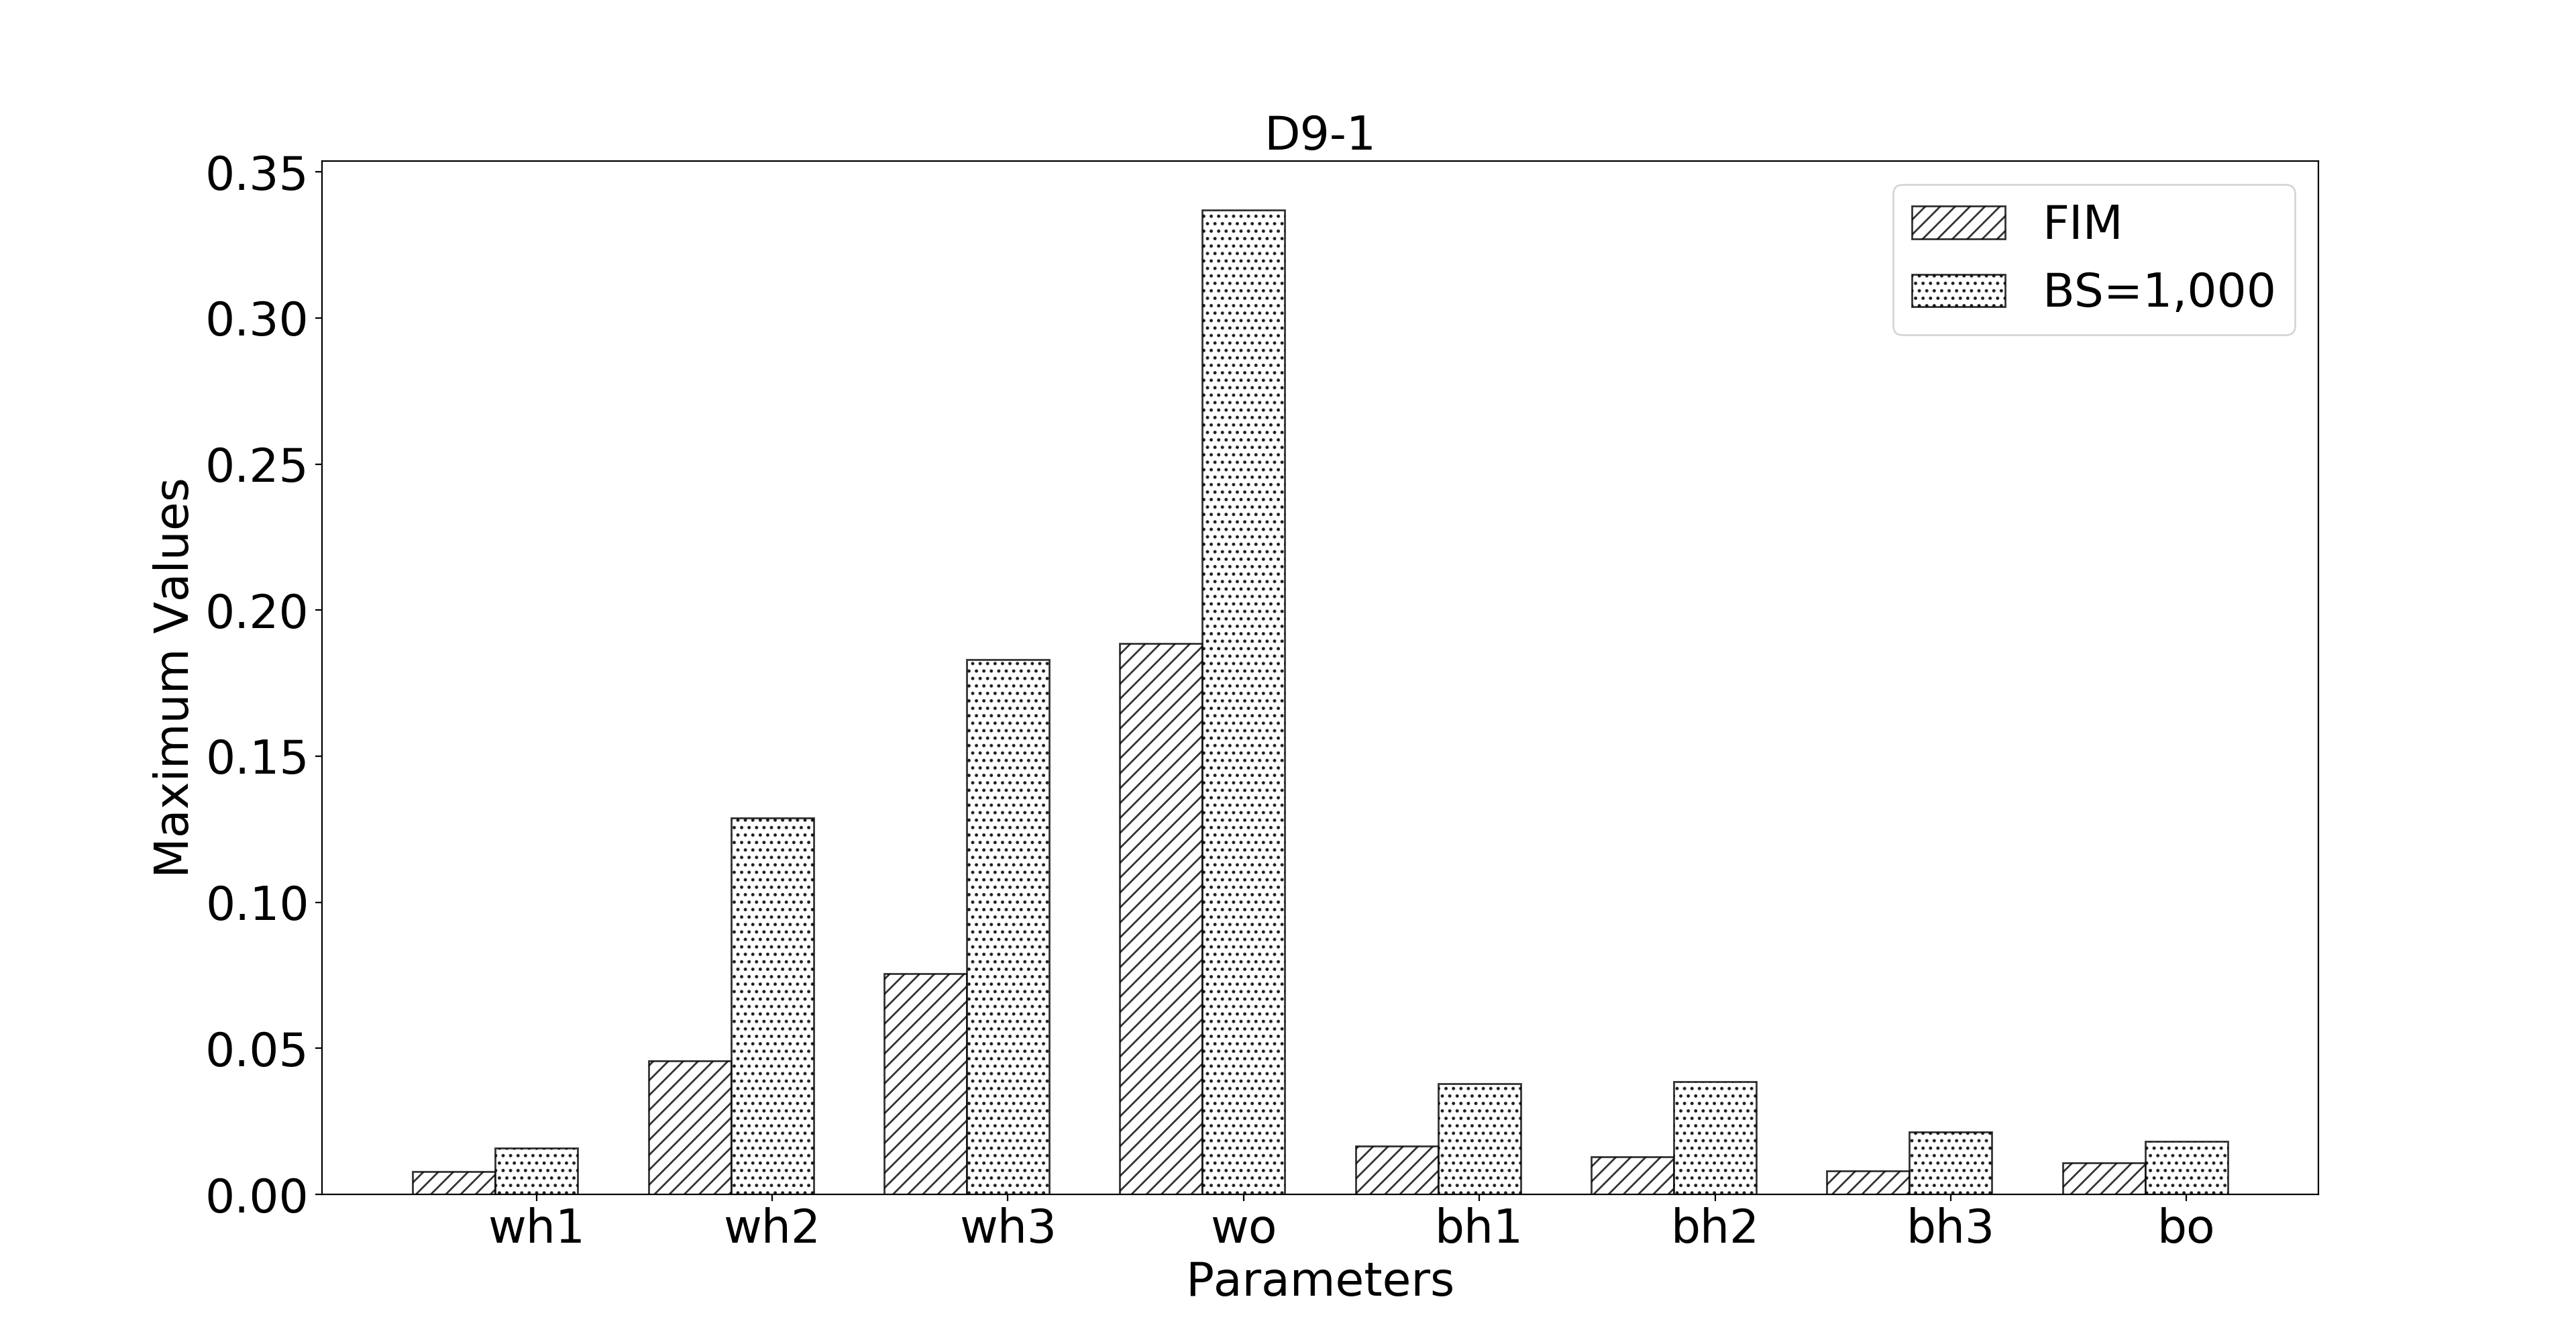
\includegraphics[width=\textwidth]{project/discussion/D91_grad_max}
    \caption{D9-1 Gradients}
    \label{fig:dis_d91}
\end{figure}

\newpage

Figure \ref{fig:ewc_d5-5} compared to Figure \ref{fig:exp_d5-5_bs1k} in the \textbf{benchmark type D5-5} are very similar.
The result of the baseline was 79.52\% and of the experiment 79.45\%, with a peak of 81.52\% compared to the experiment of 81.16\%.
So both calculations do work with the difference that the modification nearly took half the computation time of the original FIM calculation.
Figure \ref{fig:dis_d55} shows a composition of the extrem gradient values:

\begin{figure}[H]
    \centering
    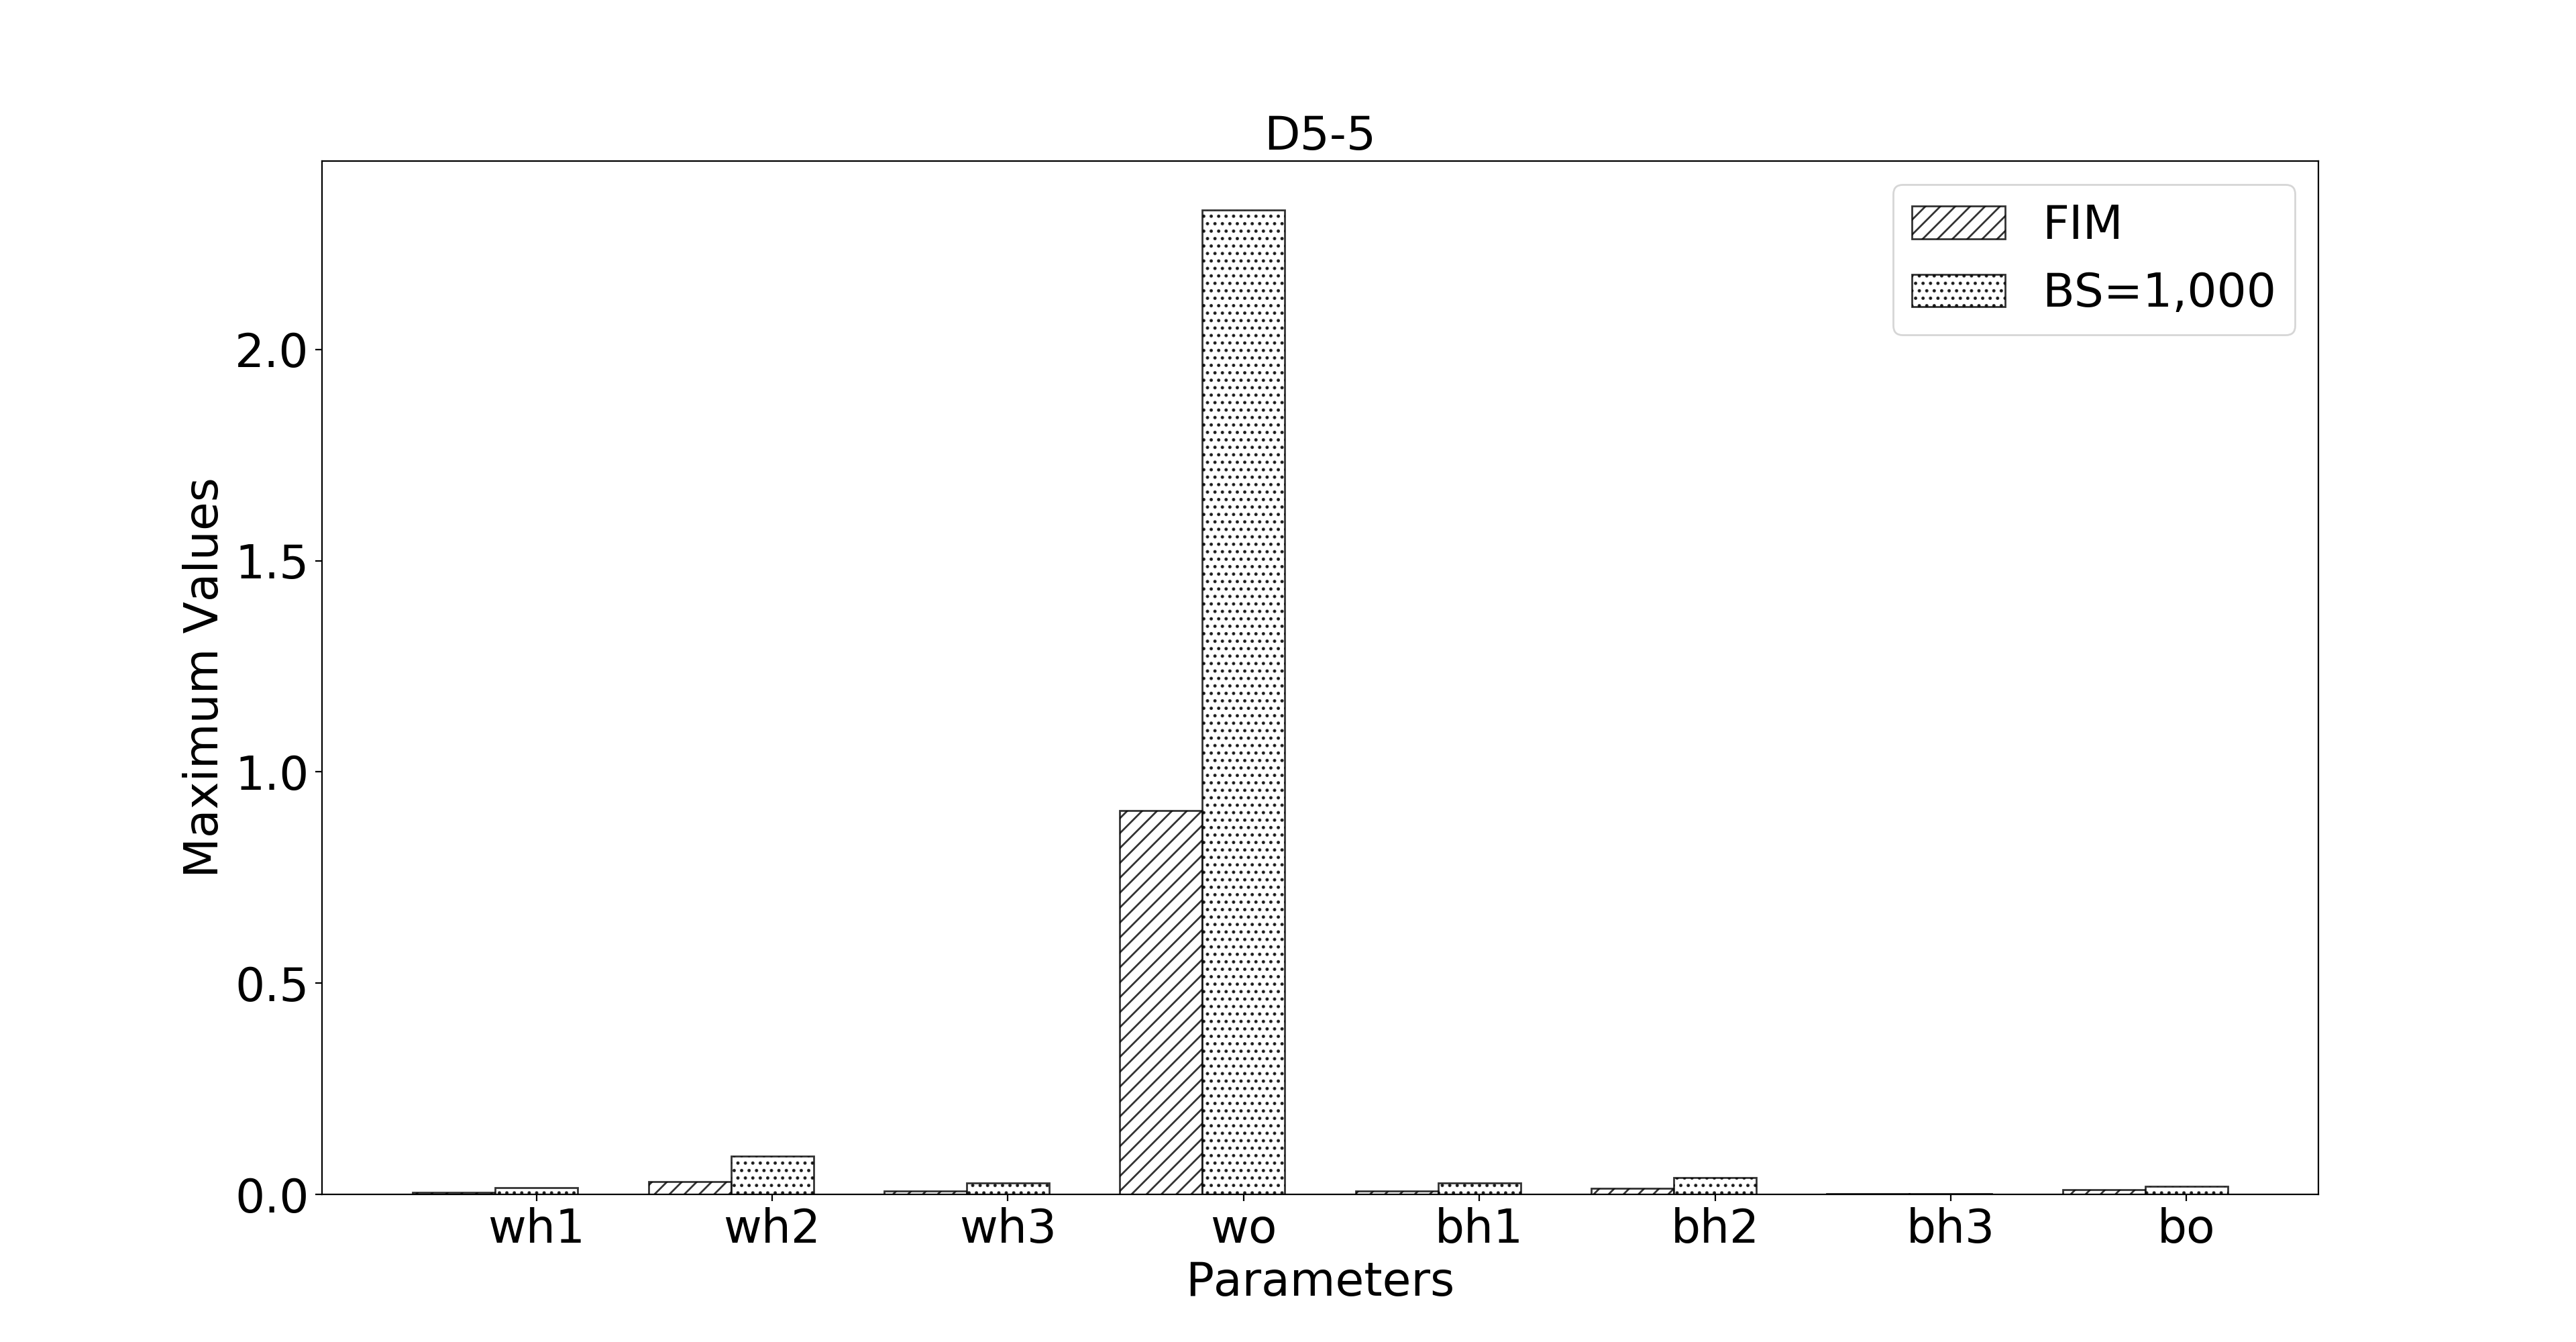
\includegraphics[width=\textwidth]{project/discussion/D55_grad_max}
    \caption{D5-5 Gradients}
    \label{fig:dis_d55}
\end{figure}

As well as the D9-1 benachmark, the gradient here show differences, but they do not make that big of a difference at the $T_2$ training.
\newline
These gradient figures of the two benchmarks (Figure \ref{fig:dis_d91}, Figure \ref{fig:dis_d55}) do show differences in the comparison of every value.
Figure \ref{fig:dis_d91} exhibits seeable more variations.
Both modifications were calculated with an average of 1,000 samples for one gradient.
But their complete size of samples and the calculated weights and bias values differs.
The D9-1 benchmarks calculated 54 averaged gradients or 54,000 per-gradients and the D5-5 benachmark 30 averaged gradients or 30,500 per-gradients.

\newpage

\textbf{Benchmark P10-10} with the baseline in Figure \ref{fig:ewc_p10-10} and the experiment Figure \ref{fig:exp_p10-10} show that both $T_2$ trainings result in the same accuracy of the complete dataset with 90.47\%.
\newline
The several tests of the modification (Table \ref{table:exp_d10-10}) show, that multiple parameter combinations of learning rate and lambda have a auspicious result.
The best results for this task are with a higher learning rate and lambda value.
\newline
Figure \ref{fig:dis_d1010} shows the comparison of the gradient maximums.
As well as the other benchmarks, the maximum values of the comparison are much higher than the maximum values of the FIM.

\begin{figure}[H]
    \centering
    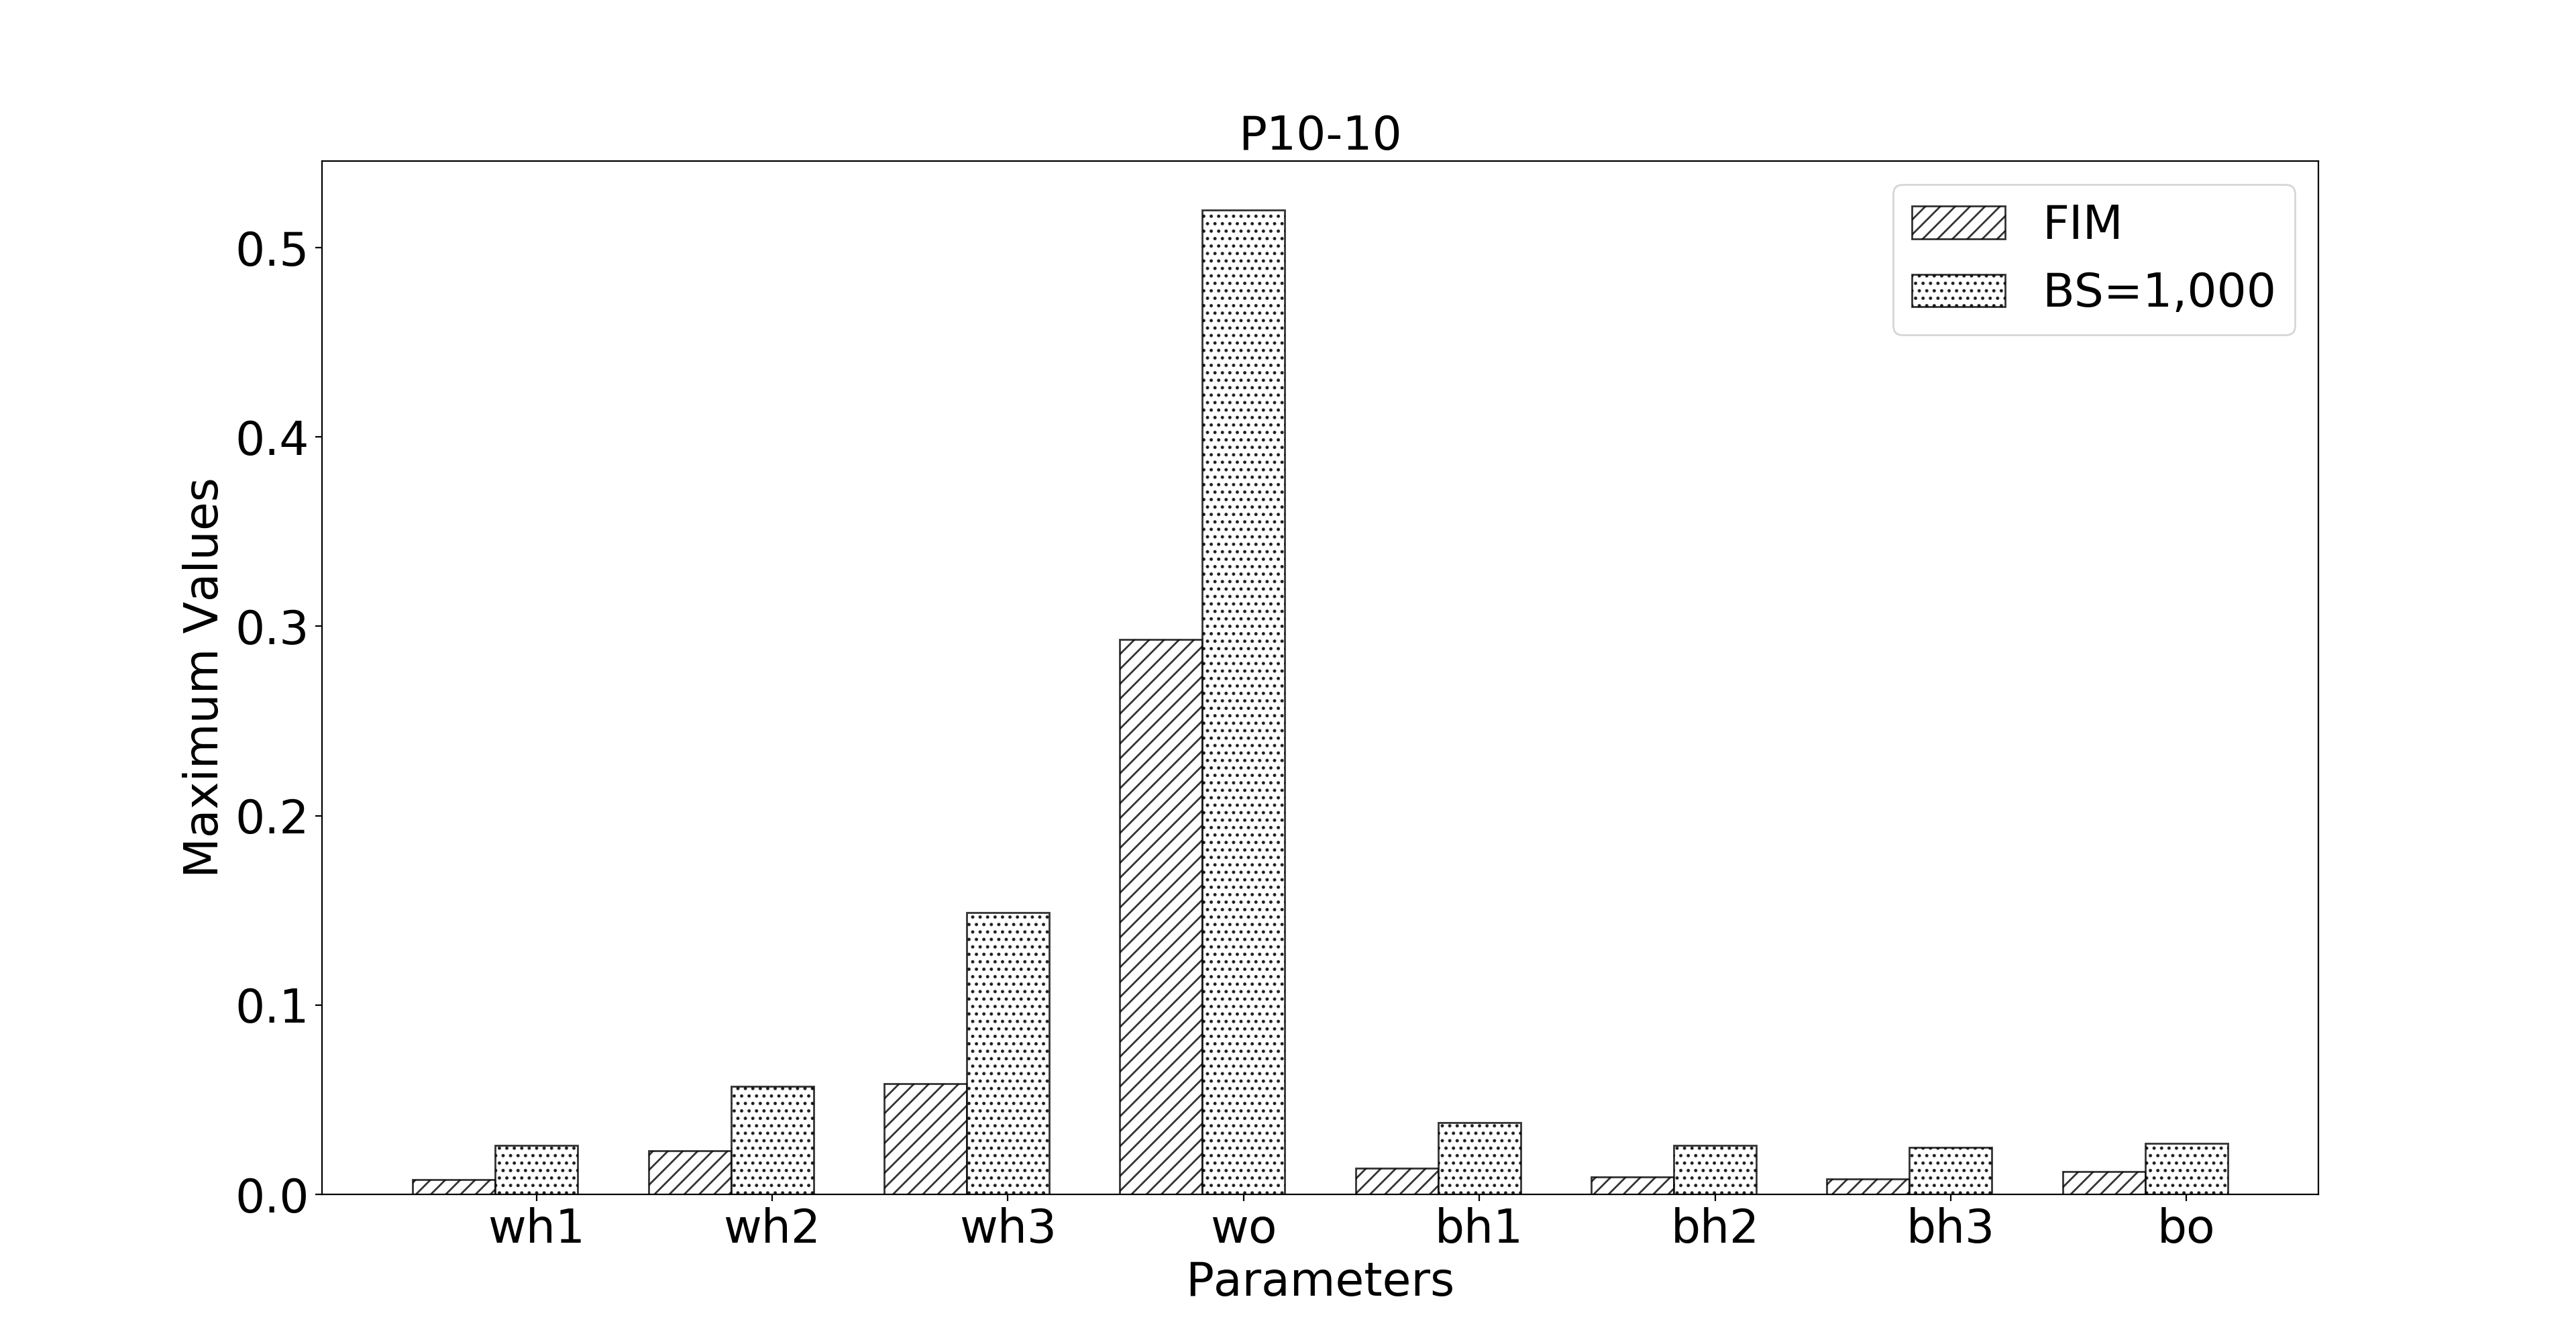
\includegraphics[width=\textwidth]{project/discussion/P1010_grad_max}
    \caption{P10-10 Gradients}
    \label{fig:dis_d1010}
\end{figure}

The promising benchmarks in this article worked with fixed iteration counts, learning rates and lambda value.
In the creation phase of the benchmarks, these three parameters had to be tested with multiple combinations.
Currently there is no solution, how to choose the quantity of iterations, learning rate or the lambda value.
So the developer needs to specify the importance of the EWC appendix.
The reference implementation set it to $\lambda = \frac{1}{learning \: rate \: T_2 }$, but we can clearly see in Table \ref{table:exp_d9-1} and Table \ref{table:exp_d5-5} of the D9-1 and D5-5 benchmarks, that this does not output the best result.
Even the comparison of these tables together show, that the chosen values for the best result differ from each other.
Regarding the tables it is important to note, that they just tested the learning rate and lambda value on a fixed iteration count.
But the number of iterations is a important component in the training process and can quickly collide with the other two parameters.
A solution for a iteration count might be the execution of a network test while training.
If the network finds a good solution while training it could presave it and train further.
If further trainings do not show a better result it can be terminated.
But this approach would definitly increase the training time, because of the increase of computations.
And it just could intercept useless training.
Overall a solution for the parameter choice problem might not be trivial.
\newline
For now the devleoper has to test multiple parameter combinations in order to find out, if this algorithm presents an useful outcome.
For every new task, a algorithm has to test multiple parameter choices in order get a feedback if there could be a promising result for the task.
This is a big problem and makes the algorithm really weak compared to the current multitask learning method.
The EWC algorithm is not predictible to get any result, but multitask learning will present a result with a measurable period, which makes it the better choice for now.

\section{Conclusion}

The experiments \& figueres from the discussion show that the modification of the FIM is a great simplification with the EWC algorithm.
It delivers very similar results compared to the EWC results from the baseline, which makes it better than the calculation of the FIM.
The computation is decreased and the algorithm alleviates catastrophic forgetting, but does not prevent it.
However, the EWC algorithm by itself deals with a lot of truble setting correct parameters.
Overall the lack of knowledge about the correct value for these parameters makes the EWC algorithm as described in their paper not useable for real-world scenarios.
So multitask learning will be the tool of choice for now.

\section{Outlook}

% test with multiple tasks and check, when the forgetting for the first task increases drastically
% just tested with fixed 2500 iterations, it should be tested with more and less iterations
% different batch sizes, because it is not per gradient anymore
% test with the modification on other datasets
% test modification on others that use fiher, like IMM or NGD
% take a closer look to lambda
%   would be useful to have a fixed lambda term
%   useless if lambda needs to be calculated for every new task…
